对CPU能力的分析表明,只要操作数在寄存器中,处理器就可以同时执行多个操作。可以计算一个相当复杂的表达式,它只依赖于两个值,所需的时间与将这些值相加所需的时间一样多。不过,依赖于两个值的限定是非常严重的限制。现在考虑一个代码示例:

\begin{lstlisting}[style=styleCXX]
for (size_t i = 0; i < N; ++i) {
	a1 += (p1[i] + p2[i])*(p1[i] - p2[i]);
}
\end{lstlisting}

所有代码都有相同的循环,只是实现更简单:\texttt{a1 += (p1[i] + p2[i]);}。同样,\texttt{p1[i]}只是\texttt{v1[i]}的别名,\texttt{p2}和\texttt{v2}也是如此。这个代码更复杂吗?处理器可以在一个周期内完成加法、减法和乘法运算,而表达式只依赖于两个值:\texttt{v1[i]}和\texttt{v2[i]},而这个表达式不能在一个循环中求值。为了明确这一点,我们引入了两个临时变量,只是表达式求值过程中的中间结果:

\begin{lstlisting}[style=styleCXX]
for (size_t i = 0; i < N; ++i) {
	s[i] = (p1[i] + p2[i]);
	d[i] = (p1[i] - p2[i]);
	a1[i] += s[i]*d[i];
}
\end{lstlisting}

如前所述,加减的结果\texttt{s[i]}和\texttt{d[i]}可以同时计算。最后一行不能执行,除非已知\texttt{s[i]}和\texttt{d[i]}的值。无论CPU一次可以做多少加法和乘法,但无法计算输入未知的操作的结果。而这里,CPU必须等待乘法的输入准备就绪。第i次迭代需要分两步执行:首先,必须加减(我们可以同时进行);其次,必须将结果相乘。迭代现在需要两个周期而不是一个周期,因为计算的第二步依赖于第一步产生的数据:

%\hspace*{\fill} \\ %插入空行
\begin{center}
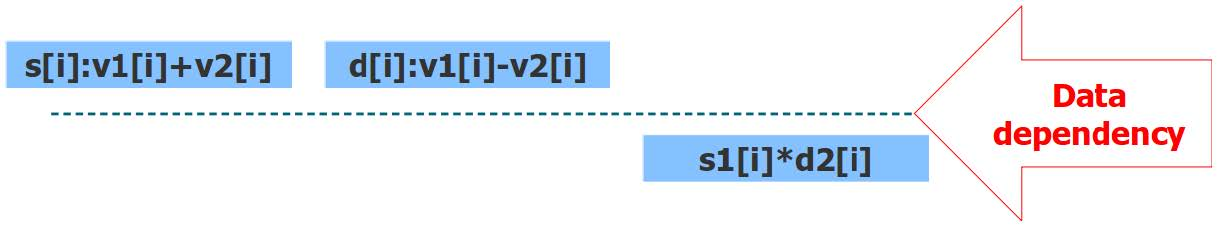
\includegraphics[width=0.8\textwidth]{content/1/chapter3/images/14.jpg}\\
图3.14 - 循环计算中的数据依赖
\end{center}

尽管CPU有资源可以同时执行这三种操作,但由于计算中的数据依赖,无法使用这种能力。当然,这严重限制了我们使用处理器的效率。依赖关系在程序中很常见,硬件设计者想出了有效的解决方案。仔细地看图3.14,当计算\texttt{s[i]}和\texttt{d[i]}的值时,乘法硬件单元闲置了。不能在更早的时候开始计算乘积,但是可以同时将之前迭代的值\texttt{s[i-1]}和\texttt{d[i-1]}相乘。现在循环的两个迭代在时间上进行交错:

%\hspace*{\fill} \\ %插入空行
\begin{center}
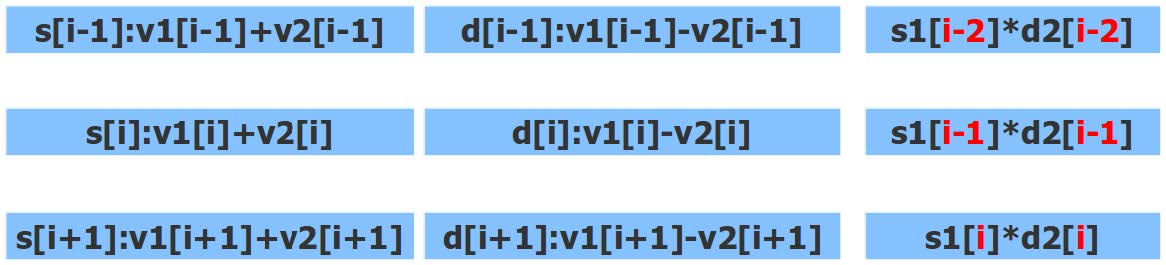
\includegraphics[width=0.8\textwidth]{content/1/chapter3/images/15.jpg}\\
图3.15 - 流水线:行对应于连续的迭代,同一行中的所有操作将同时执行
\end{center}

这种转换称为\textbf{流水线}:将复杂的表达式分解成多个阶段,并在流水线中执行。流水线中,前一个表达式的第2阶段和下一个表达式的第1阶段同时运行(更复杂的表达式将有更多的阶段,需要更深层的流水线)。只要有多次迭代,CPU就能像单次乘法那样快速地计算两阶段加减乘除的表达式:第一次迭代需要两个周期(先加减,再加减),这无法避免。类似地,最后一次迭代将以乘法结束,同时不能做其他事情,在此期间的所有迭代都会同时执行三个操作。我们已经知道CPU可以同时进行加、减、乘运算,乘法属于循环内的不同迭代。

可以用一个简单的基准测试来进行确认。这个测试中,我们将每次循环迭代做一次乘法所花费的时间,与两步迭代所花费的时间进行比较:

%\hspace*{\fill} \\ %插入空行
\begin{center}
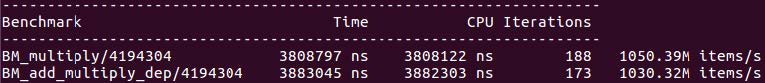
\includegraphics[width=0.9\textwidth]{content/1/chapter3/images/16.jpg}\\
图 3.16
\end{center}

正如预期,两个循环在本质上以相同的速度运行。我们可以得出结论,流水线完全消除了由数据依赖引起的性能损失。注意,流水线并没有消除数据依赖,每个循环迭代仍然必须在两个阶段执行,第二阶段取决于第一个阶段的结果。通过将不同阶段的计算交叉起来,流水线确实消除了这种依赖所致的低效率(至少在理想情况下是这样的,这也是我们目前所拥有的)。更直接的确认方式,可以从机器码分析器的结果中看到。同样,时间轴视图是最直观的:

%\hspace*{\fill} \\ %插入空行
\begin{center}
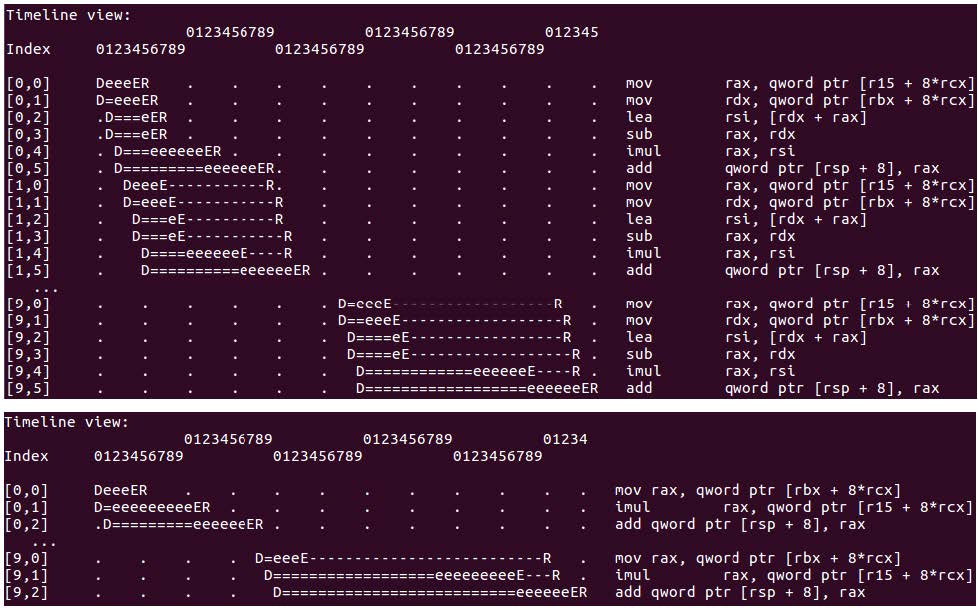
\includegraphics[width=0.9\textwidth]{content/1/chapter3/images/17.jpg}\\
图3.17 - 流水线的加减乘循环(上)和单乘法循环(下)的时间轴视图
\end{center}

如您所见,执行任一循环的10次迭代都需要56个周期。时间轴中的关键步骤是执行一条指令:\texttt{e}表示执行的开始,\texttt{E}表示执行的结束。流水线的效果在时间轴上清晰可见:循环的第一次迭代开始在第二个循环上执行,指令为[0,0],第一次迭代的最后一条指令是在第18个周期上执行的(横轴是周期数)。第二次迭代开始在第4个周期执行,两个迭代之间有明显的重叠。这就是运行中的流水线,可以看到它是如何提高程序效率的。几乎每个周期,CPU都在使用它的计算单元执行来自多次迭代的指令。执行一个简单循环所需的周期与执行更复杂循环所需的周期相同,因此额外的机器操作不需要额外的时间。

本章不打算成为机器码分析器的手册,为了更好地理解时间轴和其他信息,读者们可以自己研究一下它的文档。不过,有一个问题必须指出来,循环的每次迭代不仅执行相同的C++代码,也有完全相同的机器码。因为流水线由硬件完成,而不是编译器,编译器只为迭代生成代码,以及跳转到下一个迭代所需的操作(或完成后退出循环)。处理器并行执行多条指令,可以在时间轴上看到。经过仔细观察,有些东西是没有意义的,例如:图3.17中的指令[0,4],它在第6和12个周期期间执行,使用CPU的\texttt{rax}和\texttt{rsi}寄存器。在循环第8和9个周期期间执行的指令[1,2]:也使用相同的寄存器,写进寄存器\texttt{rsi},同时其他指令也会对寄存器\texttt{rsi}进行操作。这是不可能出现的情况,虽然CPU可以使用多个独立的计算单元同时进行多个操作,但不能同时在同一个寄存器中存储两个不同的值。尽管隐藏得很好,但这个矛盾实际上是存在的。在图3.15中,假设编译器在所有迭代中只生成一个代码副本,用来存储\texttt{s[i]}的寄存器与需要读取的\texttt{s[i-1]}使用相同寄存器,并且这两个操作同时发生。

CPU的寄存器比目前看到的要多很多。问题是每次迭代的代码完全相同,包括寄存器名称,但是在每次迭代时,必须在寄存器中存储不同的值。看起来我们的假设和流水线上的实际上情况应该不可能发生,例如:下一个迭代必须等待上一个迭代停止,使用它所需要的寄存器。但真实情况并非这样,解决这个矛盾的方法使用\textbf{寄存器重命名}的硬件技术。在程序中看到的寄存器名,例如\texttt{rsi},其实不是真正的寄存器名。可以由CPU映射到实际物理寄存器上,所以同名\texttt{rsi}可以映射到具有相同大小和功能的不同寄存器上。

当处理器在流水线中执行代码时,第一次迭代中指向\texttt{rsi}的指令实际上会使用一个内部寄存器,将其称为\texttt{rsi1}(这不是它的真实名称,但寄存器实际硬件的名称永远看不到,除非你是处理器设计师)。第二次迭代也有指向\texttt{rsi}的指令,但需要在那里存储一个不同的值,因此处理器将使用另一个寄存器\texttt{rsi2}。除非第一次迭代不再需要存储在\texttt{rsi}中的值,否则第三次迭代将不得不使用另一个寄存器,以此类推。寄存器册重命名由硬件完成,与编译器完成的寄存器分配不同(特别是,对分析代码工具不可见,如:LLVM-MCA或分析器)。最后,循环的多次迭代可以作为一个线性代码序列执行,就好像\texttt{s[i]}和\texttt{s[i+1]}使用了不同的寄存器一样。

将循环转换成线性代码称为\textbf{循环展开},这是一种流行的编译器优化技术。但这次在硬件中完成,对于能够有效地处理数据依赖关系至关重要。编译器的角度更接近于源代码的编写方式。一次迭代,一组机器指令,通过跳转到迭代的代码片段的开头反复执行。处理器的角度更像是在时间轴上看到的,一个线性指令序列,每次迭代都有自己的代码副本,并且可以使用不同的寄存器。

我们还可以观察到另一个现象,CPU执行代码的顺序实际上与指令写入的顺序并不相同。这称为乱序执行,它对多线程程序有重大影响。

我们已经了解了处理器如何规避数据依赖对执行效率的限制,其解决数据依赖的方法是流水线。然而,故事并没有在这里结束。目前为止,设计的用于执行简单循环的方案缺貌似少了一些东西,因为循环必须在某个点结束。下一节,我们将看到事情会变得多么复杂,和相应的解决方案。























